\chapter{Μέθοδος υλοποίησης}
\label{ch:implementation_method}

\section{Προτεινόμενη υλοποίηση}
Η υλοποίηση που προτείνεται στο άρθρο των \tl{Padarian J. et al}\cite{padarian_lucas_soil} αναφέρει πως δεν τροποποιεί την είσοδο στα αρχικά δεδομένα. Αυτό έχει ως αποτέλεσμα η εικόνα που προκύπτει στην είσοδο του συνελικτικού νευρωνικού δικτύου να είναι σχετικά μεγάλη. Επίσης η αρχιτεκτονική περιλαμβάνει ένα μεγάλο πλήθος επιπέδων. Ο συνδυασμός των 2 παραπάνω καθιστά την εκπαίδευση του μοντέλου ιδιαίτερα κοστοβόρα λόγω του μεγάλου πλήθους παραμέτρων.\\

Ένα επιπλέον λάθος που παρατηρείται στην συγκεκριμένη ανάλυση είναι η χρήση όλων των δειγμάτων της εδαφικής βάσης του \tl{LUCAS} συμπεριλαμβανομένων και των οργανικών δειγμάτων για ορισμένα από τα πειράματα. Αυτό οδηγεί στην εξαγωγή ορισμένων μετρικών όπως ο συντελεστής προσδιορισμού που δεν ανταποκρίνονται στην πραγματική επίδοση των μοντέλων για την ιδιότητα της περιεκτικότητας σε οργανικό άνθρακα. Το παραπάνω μπορεί να διαπιστωθεί μέσω της σύγκρισης με άλλες υλοποιήσεις με βάση την τιμή της ρίζας του μέσου τετραγωνικού σφάλματος.\\

Η προτεινόμενη υλοποίηση θα μπορούσε να τροποποιηθεί ώστε με τη χρήση ενός αντίστοιχου μοντέλου λιγότερων παραμέτρων και επιπέδων να επιτευχθεί μια παρόμοια επίδοση με τα αποτελέσματα του άρθρου των \tl{Padarian J. et al} ή να εξεταστεί ένας συνδυασμός παραμέτρων της αρχιτεκτονικής του μοντέλου ο οποίος θα οδηγήσει σε ακόμη καλύτερη επίδοση.

\section{Εργαλεία υλοποίησης}
Η ανάπτυξη των μοντέλων βαθιάς μηχανικής μάθησης και συνελικτικών νευρωνικών δικτύων έγινε στη γλώσσα \tl{Python} και με τη χρήση των σχετικών βιβλιοθηκών \tl{Tensorflow\cite{tensorflow} - Keras\cite{keras}} για το \tl{Backend} και το \tl{Frontend} αντίστοιχα για το περιβάλλον ανάπτυξης του κώδικα.

\section{Αρχιτεκτονική νευρωνικού δικτύου}
Η αρχιτεκτονική των δισδιάστατων νευρωνικών δικτύων που χρησιμοπούνται στην υλοποίηση της παρούσας διπλωματικής εργασίας έχουν μια συγκεκριμένη μορφή. Η γενική μορφή της αρχιτεκτονικής αποτελείται από τα εξής μέρη:
\begin{enumerate}
    \item Συνελικτικό επίπεδα 2 διαστάσεων
    \item Κανονικοποίηση παρτίδας
    \item Συνάρτηση ενεργοποίησης
    \item Συγκέντρωση μεγίστων
    \item Επίπεδο Dropout
    \item Πλήρως συνδεδεμένα επίπεδα
\end{enumerate}
Το βήμα συνέλιξης για τα συνελικτικά επίπεδα είναι μονάδα ενώ οι τα συνελικτικά φίλτρα διαστάσεων $3x3$ εφαρμόζονται σε όλη την έκταση της εικόνας με αναφορά το κεντρικό σημείο του συνελικτικού φίλτρου, έτσι η εικόνα εξόδου έχει ίδιες διαστάσεις με την εικόνα εισόδου στα επίπεδα της συνέλιξης.

\section{Υποδειγματοληψία φάσματος εισόδου --- αποτελεσματικότητα με ελαχιστοποίηση μεγέθους μοντέλου}
Κατά την εισαγωγή των δεδομένων του φάσματος κάθε εγγραφής εφαρμόστηκε μια μέθοδος κατά την οποία με τη χρήση μιας παραμέτρου υποδειγματοληψίας \tl{(Undersampling)} $u$ μειώνονται οι διαστάσεις των φασματικών υπογραφών. Με βάση αυτή την παράμετρο το φάσμα εισόδου δειγματοληπτείται ανά $u$ δείγματα και με τη χρήση γραμμικής παρεμβολής με τη βοήθεια της συνάρτησης \tl{interp} της βιβλιοθήκης \tl{numpy} γίνεται η εύρεση των ενδιαμέσων τιμών του διακριτού σήματος του φάσματος. Έτσι η είσοδος που προκύπτει έχει μέγεθος $\lfloor\frac{n}{u}\rfloor$. Όπου $n$ το πλήθος των δειγμάτων του φάσματος (συνήθως 4200), ενώ $u$ ο συντελεστής υποδειγματοληψίας με $u\ge1$.\\
Η επιλογή της συγκεκριμένης παραμέτρου παρατηρήθηκε πως έχει μεγάλη επιρροή στην αποτελεσματικότητα των μοντέλων. Ο λόγος για τον οποίο είναι πιθανό να συμβαίνει αυτό είναι επειδή η υποδειγματοληψία της εισόδου επηρεάζει τις τελικές διαστάσεις της εικόνας εισόδου του μοντέλου, άρα και την καταλληλότητα της εφαρμογής συνελικτικών φίλτρων συγκεκριμένων διαστάσεων σε αυτή.

\section{Μέθοδοι επίβλεψης της εκπαίδευσης του μοντέλου}
Κατά την ανάπτυξη του προτεινόμενου μοντέλου παρατηρήθηκε το φαινόμενο της "νέκρωσης" του νευρωνικού δικτύου κατά την εκπαίδευση λόγω μη ορθής αρχικοποίησης του. Το φαινόμενο αντιμετωπίστηκε με τον εντοπισμό της στασιμότητας του σφάλματος εκπαίδευσης χρησιμοποιώντας την μέση τιμή και την τυπική απόκλιση της καμπύλης εκπαίδευσης. Ο τρόπος με τον οποίο ανιχνεύεται η στασιμότητα στην εκπαίδευση είναι ο εξής, όταν μετά από ορισμένες εποχές, για παράδειγμα τρεις η τιμή του σφάλματος είναι αισθητά μεγάλη και η τυπική απόκλιση είναι σχετικά μικρή.

\subsection{Απόκλιση του σφάλματος επικύρωσης \tl{validation} κατά την εκπαίδευση}
Κατά την εκπαίδευση των δισδιάστατων νευρωνικών δικτύων παρατηρήθηκε πως το σφάλμα επικύρωσης πολλές φορές έχει σημαντική διακύμανση και η καμπύλη της εκπαίδευσης δεν έχει ομαλή εξέλιξη. Έτσι για την εξομάλυνση της διαδικασίας της εκπαίδευσης γίνεται χρήση μικρότερου ρυθμού εκμάθησης \tl{Learning Rate} από αυτόν που προτείνεται από την βιβλιοθήκη \tl{Keras}.

\subsection{Επαναρχικοποίηση εκπαίδευσης σε περίπτωση ακατάλληλων βαρών}


\subsection{Χρήση βέλτιστου μοντέλου εκπαίδευσης}
Ο σκοπός της εκπαίδευσης ενός μοντέλου είναι να αναδείξει μια εκδοχή του η οποία με τη χρήση των κατάλληλων βαρών 
Για την αξιολόγηση των μοντέλων
Ανάκτηση βέλτιστων παραμέτρων με βάση τον σφάλμα επικύρωσης
\tl{Checkpoint} μοντέλου κατά την εκπαίδευση

\subsection{Παράμετροι εκπαίδευσης}
Η εκπαίδευση οποιουδήποτε μοντέλου είναι η βασική λειτουργία που το καθιστά χρήσιμο για την εξαγωγή αποτελεσμάτων και προβλέψεων. Ο τρόπος με τον οποίο θα πραγματοποιηθεί η εκπαίδευση επηρεάζεται από ορισμένες παραμέτρους όπως ο αριθμός των εποχών, το μέγεθος παρτίδας κανονικοποίησης, ενώ η διάρκεια της θα επηρεαστεί και από την μέθοδο διασταυρωμένης επικύρωσης του επιλέγεται. Οι παραπάνω παράμετροι θα αναλυθούν στις επόμενες υποενότητες.

\subsubsection{Αριθμός εποχών}
Ο αριθμός των εποχών είναι ουσιαστικά η παράμετρος που ορίζει πόσο θα εκπαιδευτεί ένα νευρωνικό δίκτυο. Η διαδικασία της εκπαίδευσης όπως έχει αναφερθεί έχει ως σκοπό με αναδείξει ένα μοντέλο το οποίο έχει το ελάχιστο σφάλμα επικύρωσης. Κατά την την εξέλιξη της διαδικασίας της εκπαίδευσης τα σφάλματα εκπαίδευσης και επικύρωσης μειώνονται με τρόπο σχεδόν αντιστρόφως ανάλογο του αριθμού των εποχών που έχουν περάσει και έχουν κάποια διακύμανση, ενώ ο σφάλμα επικύρωσης συνήθως έχει κάποιο κατώτατο όριο το οποίο φαίνεται πως δεν είναι εφικτό να ξεπεραστεί.\\

Ως αποτέλεσμα των παραπάνω ένας μεγάλος αριθμός εποχών προσφέρει μεγαλύτερες πιθανότητες εύρεσης ενός βέλτιστου με βάση το σφάλμα επικύρωσης μοντέλου. Ωστόσο λόγω της αντιστρόφως ανάλογης σχέσης του αριθμού των εποχών και του σφάλματος τα οφέλη της εύρεσης του βέλτιστου μοντέλου αντισταθμίζονται από την μεγάλη διάρκεια της εκπαίδευσης. Επίσης μετά από ένα ορισμένο αριθμό εποχών ενδέχεται να δημιουργηθεί το φαινόμενο της υπερεκπαίδευσης.\\

Με βάση τα παραπάνω ένας βέλτιστος αριθμός εποχών είναι αυτός που προκύπτει πειραματικά ως ένα σημείο στο οποίο τα μοντέλα ελαττώνουν το σφάλμα επικύρωσης με πολύ μικρο ρυθμό ή ενδεχομένως δεν παρατηρείται καμία βελτίωση.

\begin{figure}[H]
    \begin{subfigure}{0.5\textwidth}
        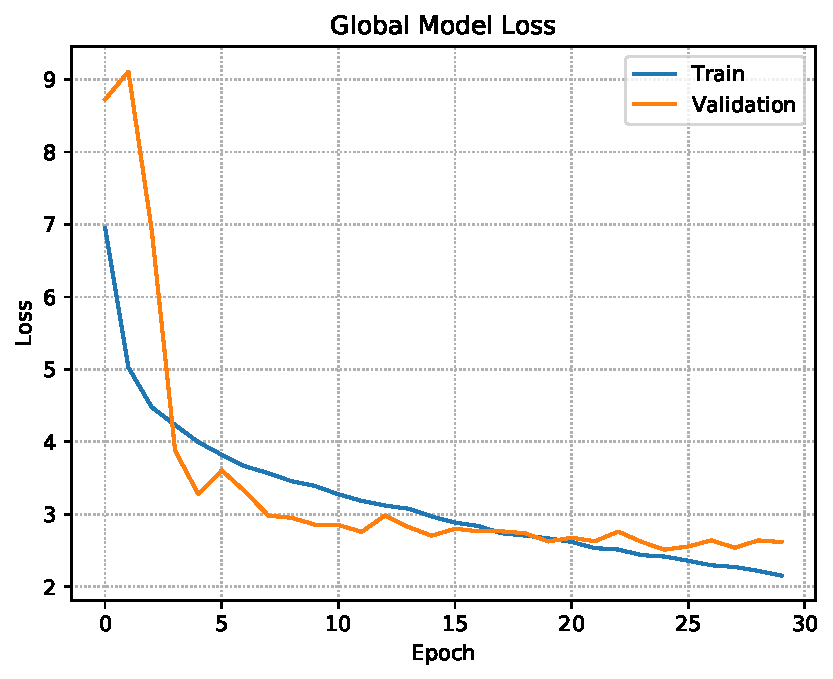
\includegraphics[width=1\linewidth]{IMPLEMENTATION_METHOD/model_loss_30_epochs.pdf}
        \caption{Διάγραμμα μείωσης του σφάλματος εκπαίδευσης και επικύρωσης για 30 εποχές}
        \label{fig:epochs30}
    \end{subfigure}
    \begin{subfigure}{0.5\textwidth}
        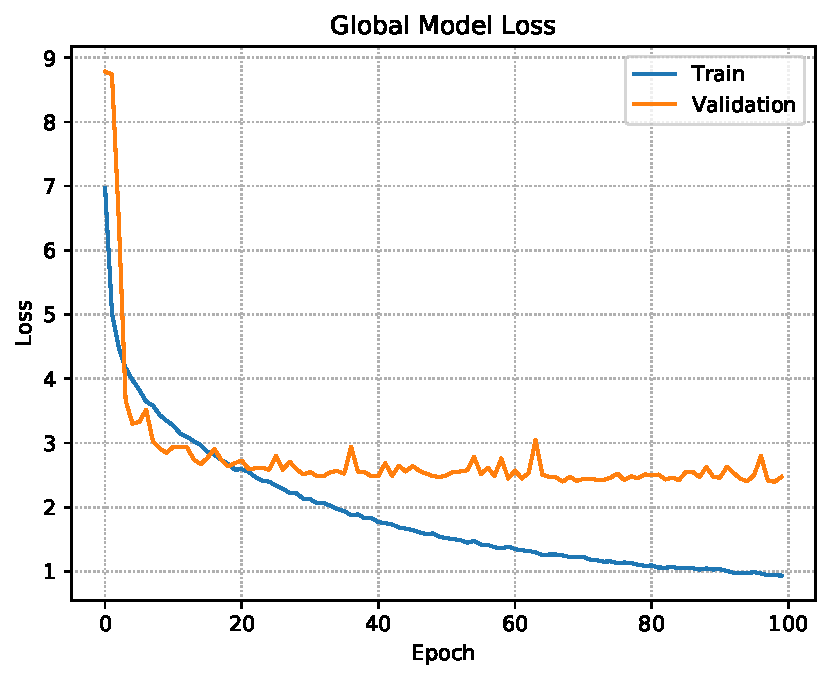
\includegraphics[width=1\linewidth]{IMPLEMENTATION_METHOD/model_loss_100_epochs.pdf}
        \caption{Διάγραμμα μείωσης του σφάλματος εκπαίδευσης και επικύρωσης για 100 εποχές}
        \label{fig:epochs100}
    \end{subfigure}
    \caption{}
\end{figure}
\begin{figure}[H]
    \centering
    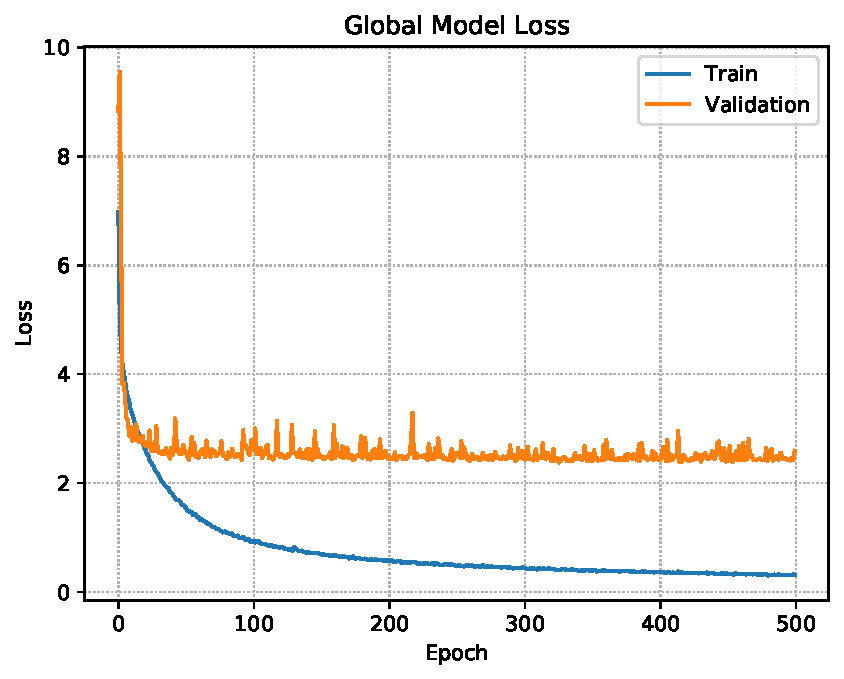
\includegraphics[width=0.5\linewidth]{IMPLEMENTATION_METHOD/model_loss_500_epochs.pdf}
    \caption{Διάγραμμα μείωσης του σφάλματος εκπαίδευσης και επικύρωσης για 500 εποχές}
    \label{fig:epochs500}
\end{figure}

Από τα παραπάνω διαγράμματα φαίνεται πως η εκπαίδευση ενός μοντέλου το οποίο αφορά το πρόβλημα της συγκεκριμένης διπλωματικής εργασίας, έχει πραγματοποιηθεί κατά ένα μεγάλο ποσοστό μετά τις 20 εποχές όπως φαίνεται στο \ref{fig:epochs30}. Ωστόσο το σφάλμα επικύρωσης μειώνεται σε αισθητό βαθμό από τις 20 εως τις 100 εποχές σύμφωνα με το \ref{fig:epochs100}. Στο \ref{fig:epochs500} φαίνεται πως η εκπαίδευση για περισσότερες από 100 εποχές μειώνει το σφάλμα επικύρωσης με πάρα πολύ αργό ρυθμό ενώ ο χρόνος εκπαίδευσης είναι δραματκά μεγαλύτερος.

\subsubsection{Μέγεθος παρτίδας κανονικοποίησης}
Το μέγεθος παρτίδας κανονικοποίησης επηρεάζει άμεσα τον τρόπο εκπαίδευσης ενός μοντέλου, άρα είναι πιθανό να επηρεάσει και την τελική επίδοση του. Ταυτόχρονα η συγκεκριμένη παράμετρος σχετίζεται άμεσα με την επιτάχυνση της εκπαίδευσης μέσω παράλληλων εργασιών με τη χρήση της κάρτας γραφικών. Ως αποτέλεσμα  το μέγεθος της παρτίδας είναι επιθυμητό να είναι ένας σχετικά μεγάλος αριθμός, συνήθως περίπου στα 64 δείγματα, ενώ στην προτεινόμενη υλοποίηση χρησιμοποιείται το μέγεθος των 32 δειγμάτων.

\subsection{Μέθοδος κ-πλης διασταυρωμένης επικύρωσης}
Κατά την εκπαίδευση των μοντέλων πάνω στο σετ δεδομένων είναι επιθυμητό να εξαλειφθεί ο παράγοντας της τυχαιότητας στον τρόπο της τελικής μορφής ενός μοντέλου και της απόδοσης του, ώστε τα τελικά αποτελέσματα να μπορούν να θεωρηθούν βάσιμα.
Οι παράγοντες οι οποίοι μπορούν να μειώσουν την τυχαιότητα και να οδηγήσουν σε ένα γενικευμένο αποτέλεσμα σε κάθε εκτέλεση του πειράματος είναι, ο αριθμός των επαναλήψεων των υπο-πειραμάτων και ο διαχωρισμός των δεδομένων σε τμήματα εκπαίδευσης--επικύρωσης--αξιολόγησης με όσο το δυνατόν διαφορετικές δομές.
Μια από τις μεθόδους επίτευξης των παραπάνω είναι η διασταυρωμένη επικύρωση. Κατά την χρήση της συγκεκριμένης μεθόδου το αρχικό σετ δεδομένων χωρίζεται σε 2 μέρη, τα δεδομένα εκπαίδευσης-επικύρωσης και τα δεδομένα αξιολόγησης τα οποία χρησιμοποιούνται έπειτα από την διαδικασία εκπαίδευσης. Τα 2 αυτά μέρη είναι χωρισμένα με ποσοστά πτυχών 60 -- 40 \% με περίπου 12000 από τα 19000 δείγματα. Το μέρος εκπαίδευσης-επικύρωσης του σετ δεδομένων χωρίζεται στα επιμέρους τμήματα του σε ποσοστά 80 -- 20 \% αντίστοιχα, με περίπου 9566 και 2392 δείγματα.
Η διαδικασία διαχωρισμού των τμημάτων εκπαίδευσης-επικύρωσης του σετ δεδομένων επαναλαμβάνεται χρησιμοποιώντας κάθε φορά μια διαφορετική από τις 5 πτυχές διαχωρισμού ως το σετ επικύρωσης.

Αυτό που επιτυγχάνεται ουσιαστικά είναι η εξαγωγή μετρικών με τη χρήση των προβλέψεων 5 διαφορετικών μοντέλων

\section{Τροποποίηση αρχιτεκτονικής προτεινόμενου μοντέλου}
Κατά την διαδικασία εύρεσης ενός μοντέλου με τα βέλτιστα χαρακτηριστικά εξετάζονται ορισμένες τροποποιήσεις της αρχιτεκτονικής του μέσω της χρήσης διαφορετικών μεγεθών των παραμέτρων των επιπέδων ή της παράλειψης επιπέδων ή χρήση άλλων που δεν υπάρχουν στην προτεινόμενη υλοποίηση. Τα πειράματα τα οποία πραγματοποιήθηκαν με σκοπό την εύρεση του βέλτιστου μοντέλου θα αναλυθούν στο κεφάλαιο \ref{ch:experiments_and_results}

\section{Μοντέλο μιας εισόδου -- μιας εξόδου}
Η βασική υλοποίηση του προτεινόμενου μοντέλου αφορά ένα μοντέλο μιας εισόδου και μιας εξόδου. Με τη συγκεκριμένη αρχιτεκτονική μοντέλου γίνεται απόπειρα πρόβλεψης μιας εδαφικής ιδιότητας με τη χρήση ενός σπεκτρογράμματος και αποτελεί την απλούστερη αρχιτεκτονική δισδιάστατου συνελικτικού νευρωνικού δικτύου για την λύση αυτού του προβλήματος.
\begin{figure}[H]
  \begin{center}
    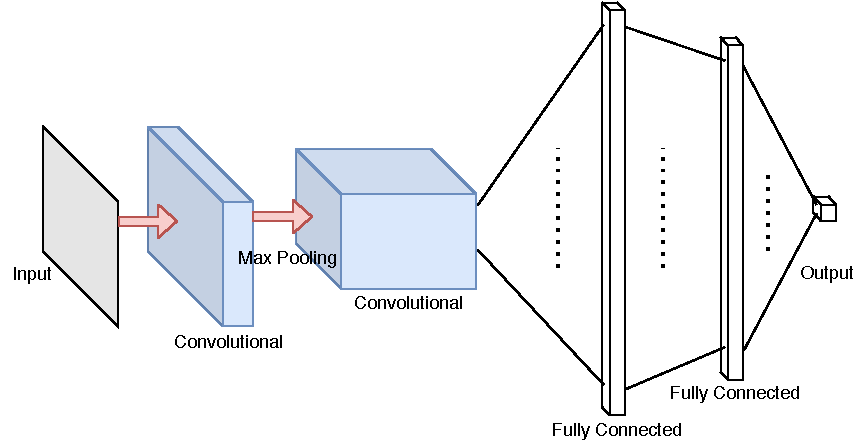
\includegraphics[width=1\textwidth]{IMPLEMENTATION_METHOD/model_SI-SO.pdf}
    \caption{Αρχιτεκτονική του μοντέλου μιας εισόδου---μιας εξόδου}
  \end{center}
\end{figure}
\section{Μοντέλο πολλαπλών εξόδων}
Μια δεύτερη υλοποίηση προτεινόμενου μοντέλου είναι η εξέλιξη του πρώτου μοντέλου σε ένα το οποίο θα εκτελεί πολλαπλές προβλέψεις ιδιοτήτων. Στην αρχιτεκτονική του μοντέλου υπάρχει η διαφορά πως διαθέτει πολλές εξόδους. Το σημείο στο οποίο δημιουργούνται οι πολλαπλές διεργασίες του μοντέλου είναι πριν από τα πλήρως συνδεδεμένα επίπεδα. Ένα μοντέλο το οποίο διαθέτει παραπάνω από μια εξόδους θεωρείται πως κατά την εκπαίδευση λαμβάνει πολυδιάστατες αναδράσεις σχετικά με τα σφάλματα πρόβλεψης του και ως αποτέλεσμα εκπαιδεύεται με πιο σφαιρικό τρόπο από ένα μοντέλο μιας εξόδου. Ωστόσο μια διαφορά σε σχέση με το μοντέλο μιας εξόδου είναι πως η επιλογή του βέλτιστου μοντέλου γίνεται με βάση το άθροισμα των σφαλμάτων επικύρωσης έτσι δεν είναι δεδομένο πως το μοντέλο θα έχει την βέλτιστη επίδοση για όλες τις ιδιότητες του σε αντίθεση με το δεύτερο στο οποίο για κάθε έξοδο γίνεται η εύρεση του βέλτιστου μοντέλου.

\begin{figure}[H]
  \begin{center}
    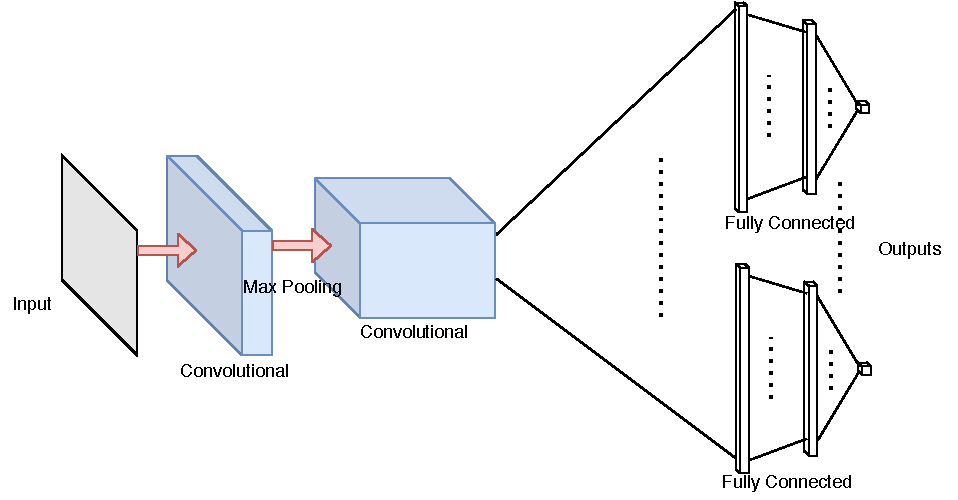
\includegraphics[width=1\textwidth]{IMPLEMENTATION_METHOD/model_SI-MO.pdf}
    \caption{Αρχιτεκτονική του μοντέλου μιας εισόδου---πολλαπλών εξόδων}
  \end{center}
\end{figure}

\section{Μοντέλο πολλαπλών εισόδων -- εξόδων}
Κατά την δοκιμή των πιθανών αρχιτεκτονικών που δοκιμάστηκαν έγινε η υπόθεση πως ένα μοντέλο το οποίο θα λαμβάνει πολλαπλά σπεκτρογράμματα μετασχηματισμών της εισόδου είναι πιθανό να έχει καλύτερη από ένα απλό μοντέλο μιας εισόδου. Η υπόθεση αυτή βασίζεται στην παρατήρηση πως για τις 2 διαφορετικές εισόδους της ανακλαστικότητας και της 1ης παραγώγου του μετασχηματισμού  \tl{Savitzky-Golay} της απορροφητικότητας το μοντέλο παρουσιάζει βέλτιστη επίδοση για διαφορετικές εξόδους σε κάθε είσοδο. Έτσι υποτίθεται πως η χρήση πολλαπλών εισόδων και εξόδων θα δύναται να παρέξει πληροφορία για την εξαγωγή των βέλτιστων προβλέψεων για όλες τις ιδιότητες εδάφους ενώ η εκπαίδευση του μοντέλου ευνοείται από τη χρήση πολλαπλών εξόδων.

\begin{figure}[H]
  \begin{center}
    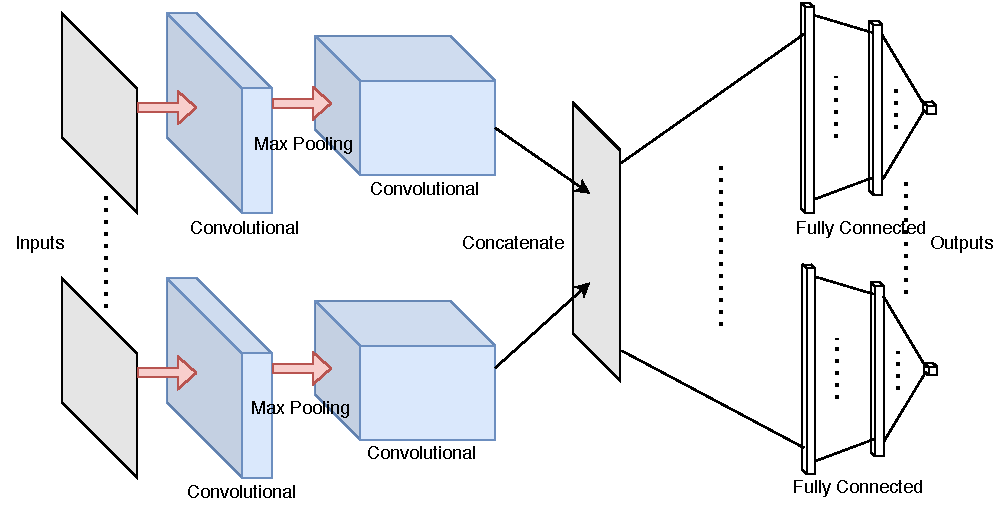
\includegraphics[width=1\textwidth]{IMPLEMENTATION_METHOD/model_MI-MO.pdf}
    \caption{Αρχιτεκτονική του μοντέλου πολλαπλών εισόδων---πολλαπλών εξόδων}
  \end{center}
\end{figure}

\section{Μοντέλο πολλαπλών εισόδων -- μιας εξόδου}
Στη συγκεκριμένη αρχιτεκτονική όπως και στην προηγούμενη υποενότητα γίνεται χρήση της πληροφορίας που παρέχεται από τις πολλαπλές εισόδους ενώ η εύρεση του βέλτιστου μοντέλου πραγματοποιείται με γνώμονα μια εδαφική ιδιότητα.
\begin{figure}[H]
  \begin{center}
    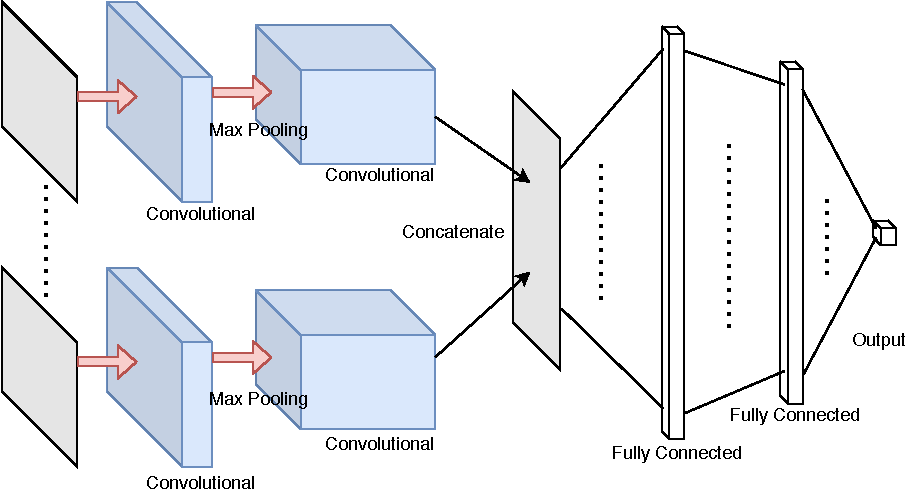
\includegraphics[width=1\textwidth]{IMPLEMENTATION_METHOD/model_MI-SO.pdf}
    \caption{Αρχιτεκτονική του μοντέλου πολλαπλών εισόδων---μιας εξόδου}
  \end{center}
\end{figure}
\section{Υλοποίηση εξαγωγής 1η παραγώγου μετασχηματισμού \tl{Savitzky Golay} απορροφητικότητας από ανακλαστικότητα}
Πρόλογος\\
Για εξαγωγή του συγκεκριμένου μετασχηματισμού αρχικά οι φασματικές υπογραφές ανακλασικότητας μετατρέπονται σε απορροφητικότητες. Η παραπάνω μετατροπή γίνεται με την εφαρμογή του παραπάνω τύπου στο φάσμα.
$$Absorbance=-log_{10}(Reflectance)$$

Η μορφή της φασματικής υπογραφής πριν και μετά την μετατροπή σε απορροφητικότητα φαίνεται στα σχήματα \ref{fig:abs_sg1_initial} και \ref{fig:abs_sg1_abs} αντίστοιχα.\\

Μετά τον μετασχηματισμό \tl{Savitzky-Golay} φαίνεται πως η φασματική υπογραφή έχει μεγάλες τιμές για τα αρχικά της δείγματα λόγω της μεγάλης κλίσης της φασματικής υπογραφής, κάτι που θα εισάγει μεγάλες τιμές στο δισδιάστατο συνελικτικό νευρωνικό δίκτυο για εκείνη την περιοχή του σήματος οι οποίες είναι πολύ μεγαλύτερες απο τις διακυμάνσεις σε όλη την υπόλοιπη έκταση του. Επίσης το εύρος τιμών της είναι πολύ μικρό σε σχέση με σχέση με τις τιμές της ανακλαστικότητας. Για την επίλυση των παραπάνω προβλημάτων αρχικά γίνεται κανονικοποίηση του φάσματος πολλαπλασιάζοντας την είσοδο με 333 και προσθέτοντας 0.5, έτσι το εύρος τιμών του μετασχηματισμένου σήματος είναι ίδιο με το αρχικό που έχει ανακλαστικότητα. Επίσης για την διόρθωση των ακραίων τιμών στα πρώτα δείγματα του σήματος εφαρμόζεται μια μάσκα για τον περιορισμό των τιμών στα πρώτα 100 δείγματα.\\
Ο τύπος του μετασχηματισμού για τα 100 πρώτα δείγματα είναι ο εξής:
\[
    y[i]= 
\begin{cases}
    333\left(\frac{i}{100}\right)^{1,6}x[i]+0,5,& 0\leq x<100\\
    333 x[i]+0,5,              & 100\leq x<4200
\end{cases}
\]
Όπου $x[i]$ το δείγμα $i$ του φάσματος μετά τον μετασχηματισμό \tl{Savitzky-Golay} και $y[i]$ η τελική μορφή του σήματος.\\

Η μορφή της φασματικής υπογραφής όταν μετά τον μετασχηματισμό \tl{Savitzky-Golay} και τελικά μετά την κανονικοποίηση και την διόρθωση των αρχικών φαίνεται στα σχήματα \ref{fig:abs_sg1_transform_notches} και \ref{fig:abs_sg1_transform_fixed} αντίστοιχα.\\

\begin{figure}[H]
    \begin{subfigure}{0.5\textwidth}
        \includesvg[width=1\linewidth]{IMPLEMENTATION_METHOD/0_Initial}
        \caption{Αρχική μορφή φασματικής υπογραφής ανακλαστικότητας}
        \label{fig:abs_sg1_initial}
    \end{subfigure}
    \begin{subfigure}{0.5\textwidth}
        \includesvg[width=1\linewidth]{IMPLEMENTATION_METHOD/0_Abs}
        \caption{Μορφή φασματικής υπογραφής μετά τη μετατροπή σε απορροφητικότητα}
        \label{fig:abs_sg1_abs}
    \end{subfigure}
    \begin{subfigure}{0.5\textwidth}
        \includesvg[width=1\linewidth]{IMPLEMENTATION_METHOD/0_Abs_SG1}
        \caption{Φασματική υπογραφή μετά στον μετασχηματισμό \tl{}}
        \label{fig:abs_sg1_transform_notches}
    \end{subfigure}
    \begin{subfigure}{0.5\textwidth}
        \includesvg[width=1\linewidth]{IMPLEMENTATION_METHOD/0_Abs_SG1_Fixed}
        \caption{Μορφή φασματικής υπογραφής μετά τη μετατροπή σε απορροφητικότητα}
        \label{fig:abs_sg1_transform_fixed}
    \end{subfigure}
    \caption{Απεικόνιση φασματικής υπογραφής κατά τα στάδια της μετατροπής της σε μετασχηματισμό \tl{Savitzky-Golay} πρώτης παραγώγου}
\end{figure}


\section{Κανονικοποίηση δεδομένων εισόδου -- εξόδου}
Τα δεδομένα τα οποία θα εισαχθούν στο δισδιάστατο νευρωνικό δίκτυο θεωρείται πως είναι βέλτιστο να έχουν μια κατανομή η οποία θα οδηγεί σε παρόμοια εύρη τιμών, έτσι επιλέγεται η κανονικοποίηση με χρήση της μέσης τιμής και της διακύμανσης του εκάστοτε συνόλου. Με την τεχνική που χρησιμοποιείται τα δεδομένα έχουν μέση τιμή μηδέν και διακύμανση μονάδα.

\subsection{Κανονικοποίηση εισόδου}
Η είσοδος που προκύπτει από την μετασχηματισμό \tl{Fourier} βραχέως χρόνου είναι σε κλίμακα με μικρού εύρος τιμών και μικρής τάξης μεγέθους έτσι είναι απαραίτητη η χρήση της λογαριθμικής για την διάκριση των τιμών της εικόνας. Το αποτέλεσμα που προκύπτει μετά την λογαρίθμηση έχει σχετικά μεγάλες τιμές με εύρος $~[0,50]$, οπότε γίνεται κανονικοποίηση των τιμών στο διάστημα $[-1,1]$ όπως αναφέρεται παραπάνω ώστε να είναι σε μορφή εύχρηστη για την εισαγωγή τους στην είσοδο του δισδιάστατου συνελικτικού νευρωνικού δικτύου.
\subsection{Κανονικοποίηση εξόδου}
Ένας βασικός λόγος που η έξοδος κανονικοποιείται με μέση τιμή μηδέν και διακύμανση μονάδα είναι ώστε τα σφάλματα που προκύπτουν κατά την εκπαίδευση των μοντέλων πολλών εξόδων να είναι ισοδύναμα, ώστε να μην επιλέγεται κάποιο μοντέλο με βάση την βελτίωση της επίδοσης του σε μια συγκεκριμένη ιδιότητα.